\RequirePackage{fix-cm}
\documentclass[twoside,twocolumn,9pt]{extarticle}
\usepackage[super,sort&compress,comma]{natbib}
\usepackage[version=3]{mhchem}
\usepackage[left=1.5cm, right=1.5cm, top=1.785cm, bottom=2.0cm]{geometry}
\usepackage{balance}
\usepackage{mathptmx}
\usepackage{graphicx}
\usepackage{lastpage}
\usepackage[format=plain,justification=justified,singlelinecheck=false,font={stretch=1.125,small,sf},labelfont=bf,labelsep=space]{caption}
\usepackage{float}
\usepackage{fancyhdr}
\usepackage{fnpos}
\usepackage[english]{babel}
\addto{\captionsenglish}{%
  \renewcommand{\refname}{Notes and references}
}
\usepackage{array}
\usepackage{charter}
\usepackage[T1]{fontenc}
\DeclareFontSeriesDefault[sf]{bf}{bx}
\usepackage[dvipsnames]{xcolor}
\usepackage{setspace}
\usepackage[compact]{titlesec}
\usepackage{amsmath}
\usepackage{amssymb}
\usepackage{amsthm}
\usepackage{booktabs}
\usepackage{xr}
\usepackage[hidelinks,hyperfootnotes=false]{hyperref}
\externaldocument[E-]{esi}

\newtheorem{theorem}{Theorem}
\newtheorem{remark}{Remark}

\definecolor{cream}{RGB}{222,217,201}

\renewcommand{\dbltopfraction}{0.95}
\renewcommand{\dblfloatpagefraction}{0.6}
\renewcommand{\topfraction}{0.9}
\renewcommand{\floatpagefraction}{0.6}
\setcounter{dbltopnumber}{3}
\setcounter{topnumber}{3}

\begin{document}

\pagestyle{fancy}
\thispagestyle{plain}
\fancypagestyle{plain}{
\renewcommand{\headrulewidth}{0pt}
}

\makeFNbottom
\makeatletter
\renewcommand\LARGE{\@setfontsize\LARGE{15pt}{17}}
\renewcommand\Large{\@setfontsize\Large{12pt}{14}}
\renewcommand\large{\@setfontsize\large{10pt}{12}}
\renewcommand\footnotesize{\@setfontsize\footnotesize{7pt}{10}}
\makeatother

\renewcommand{\thefootnote}{\fnsymbol{footnote}}
\renewcommand\footnoterule{\vspace*{1pt}%
\color{cream}\hrule width 3.5in height 0.4pt \color{black}\vspace*{5pt}}
\setcounter{secnumdepth}{3}

\makeatletter
\renewcommand\@biblabel[1]{#1}
\renewcommand\@makefntext[1]%
{\noindent\makebox[0pt][r]{\@thefnmark\,}#1}
\makeatother
\renewcommand{\figurename}{\small{Fig.}~}
\titleformat*{\section}{\normalfont\sffamily\Large}
\titleformat*{\subsection}{\normalfont\normalsize\bfseries}
\titleformat*{\subsubsection}{\normalfont\normalsize\bfseries}
\setstretch{1.125}
\setlength{\skip\footins}{0.8cm}
\setlength{\footnotesep}{0.25cm}
\setlength{\jot}{10pt}
\titlespacing*{\section}{0pt}{4pt}{4pt}
\titlespacing*{\subsection}{0pt}{15pt}{1pt}

\fancyfoot{}
\fancyfoot[LO,RE]{\vspace{-7.1pt}
\includegraphics[height=9pt]{head_foot/LF.pdf}}
\fancyfoot[CO]{\vspace{-7.1pt}\hspace{13.2cm}
\includegraphics{head_foot/RF.pdf}}
\fancyfoot[CE]{\vspace{-7.2pt}\hspace{-14.2cm}
\includegraphics{head_foot/RF.pdf}}
\fancyfoot[RO]{\footnotesize{\sffamily{1--\pageref{LastPage} ~\textbar  \hspace{2pt}\thepage}}}
\fancyfoot[LE]{\footnotesize{\sffamily{\thepage~\textbar\hspace{3.45cm} 1--\pageref{LastPage}}}}
\fancyhead{}
\renewcommand{\headrulewidth}{0pt}
\renewcommand{\footrulewidth}{0pt}
\setlength{\arrayrulewidth}{1pt}
\setlength{\columnsep}{6.5mm}
\setlength\bibsep{1pt}

\makeatletter
\newlength{\figrulesep}
\setlength{\figrulesep}{0.5\textfloatsep}
\newcommand{\topfigrule}{\vspace*{-1pt}%
\noindent{\color{cream}\rule[-\figrulesep]{\columnwidth}{1.5pt}} }
\newcommand{\botfigrule}{\vspace*{-2pt}%
\noindent{\color{cream}\rule[\figrulesep]{\columnwidth}{1.5pt}} }
\newcommand{\dblfigrule}{\vspace*{-1pt}%
\noindent{\color{cream}\rule[-\figrulesep]{\textwidth}{1.5pt}} }
\makeatother
\renewcommand{\dblfigrule}{}

\twocolumn[
  \begin{@twocolumnfalse}
{
\includegraphics[height=30pt]{head_foot/journal_name.pdf}\hfill\raisebox{0pt}[0pt][0pt]{
\includegraphics[height=55pt]{head_foot/RSC_LOGO_CMYK.pdf}}\\[1ex]

\includegraphics[width=18.5cm]{head_foot/header_bar.pdf}}\par
\vspace{1em}
\sffamily
\begin{tabular}{m{4.5cm} p{\dimexpr\textwidth-4.5cm-4\tabcolsep\relax}}


\includegraphics{head_foot/DOI.pdf} & \noindent\LARGE{\textbf{Geometric algebra meets Cartesian tensors: higher-order equivariance for interatomic potentials$^\dag$}} \\
\vspace{0.3cm} & \vspace{0.3cm} \\

 & \noindent\large{Can Polat,\textit{$^{a}$} Mustafa Kurban,$^{\ast}$\textit{$^{bc}$} Erchin Serpedin\textit{$^{a}$} and Hasan Kurban$^{\ast}$\textit{$^{d}$}} \\


\includegraphics{head_foot/dates.pdf} & \noindent\normalsize{Clifford-algebra interatomic potentials offer a compact equivariant representation, but their three-dimensional multivectors contain only scalar and vector angular channels ($L=0,1$), leaving higher-order channels absent. We investigate whether explicitly supplying these missing channels improves the accuracy of predicted force directions. We introduce CliffordSTF, which couples Clifford multivectors to symmetric traceless tensors of ranks two and three ($L=2,3$) through closed-form generation and contraction operations, extending their angular representation while retaining geometric-product message passing. The construction supplies explicit higher-order angular features without spherical-harmonic tensor products or Clebsch--Gordan tables. CliffordSTF increases aggregate force cosine similarity on revised MD17 by a factor of $10.0$ and reduces force mean absolute error by $13.9\%$ relative to the base model, with lower force error on all ten molecules and unchanged aggregate energy error at the reported precision. An ablation of eleven variants plus the baseline identifies the rank-2 edge descriptor as the main source of the directional gain. On the OC20 catalyst dataset, results show improved relaxed-energy and force prediction over the base model, while transfer to OC22 is mixed. These results demonstrate a route to higher-order angular features within a Clifford potential and identify which additions drive its improved force predictions.} \\

\end{tabular}

 \end{@twocolumnfalse} \vspace{0.6cm}

  ]

\renewcommand*\rmdefault{bch}\normalfont\upshape
\rmfamily
\section*{}
\vspace{-1cm}

\footnotetext{\textit{$^{a}$~Department of Electrical and Computer Engineering, Texas A\&M University, College Station, Texas, USA. ORCID: Can Polat 0000-0002-1458-302X; Erchin Serpedin 0000-0001-9069-770X.}}
\footnotetext{\textit{$^{b}$~Department of Electrical and Computer Engineering, Texas A\&M University at Qatar, Doha, Qatar.}}
\footnotetext{\textit{$^{c}$~Department of Prosthetics and Orthotics, Ankara University, Ankara, Turkey. E-mail: kurbanm@ankara.edu.tr. ORCID: Mustafa Kurban 0000-0002-7263-0234.}}
\footnotetext{\textit{$^{d}$~College of Science and Engineering, Hamad Bin Khalifa University, Doha, Qatar. E-mail: hkurban@hbku.edu.qa. ORCID: Hasan Kurban 0000-0003-3142-2866.}}
\footnotetext{\dag~Electronic supplementary information (ESI) available: algebraic derivations, architecture and training details, complete benchmark and ablation results, per-seed analyses, and computational measurements.}

\section{Introduction}\label{sec:intro}

\begin{figure*}[t]
\centering
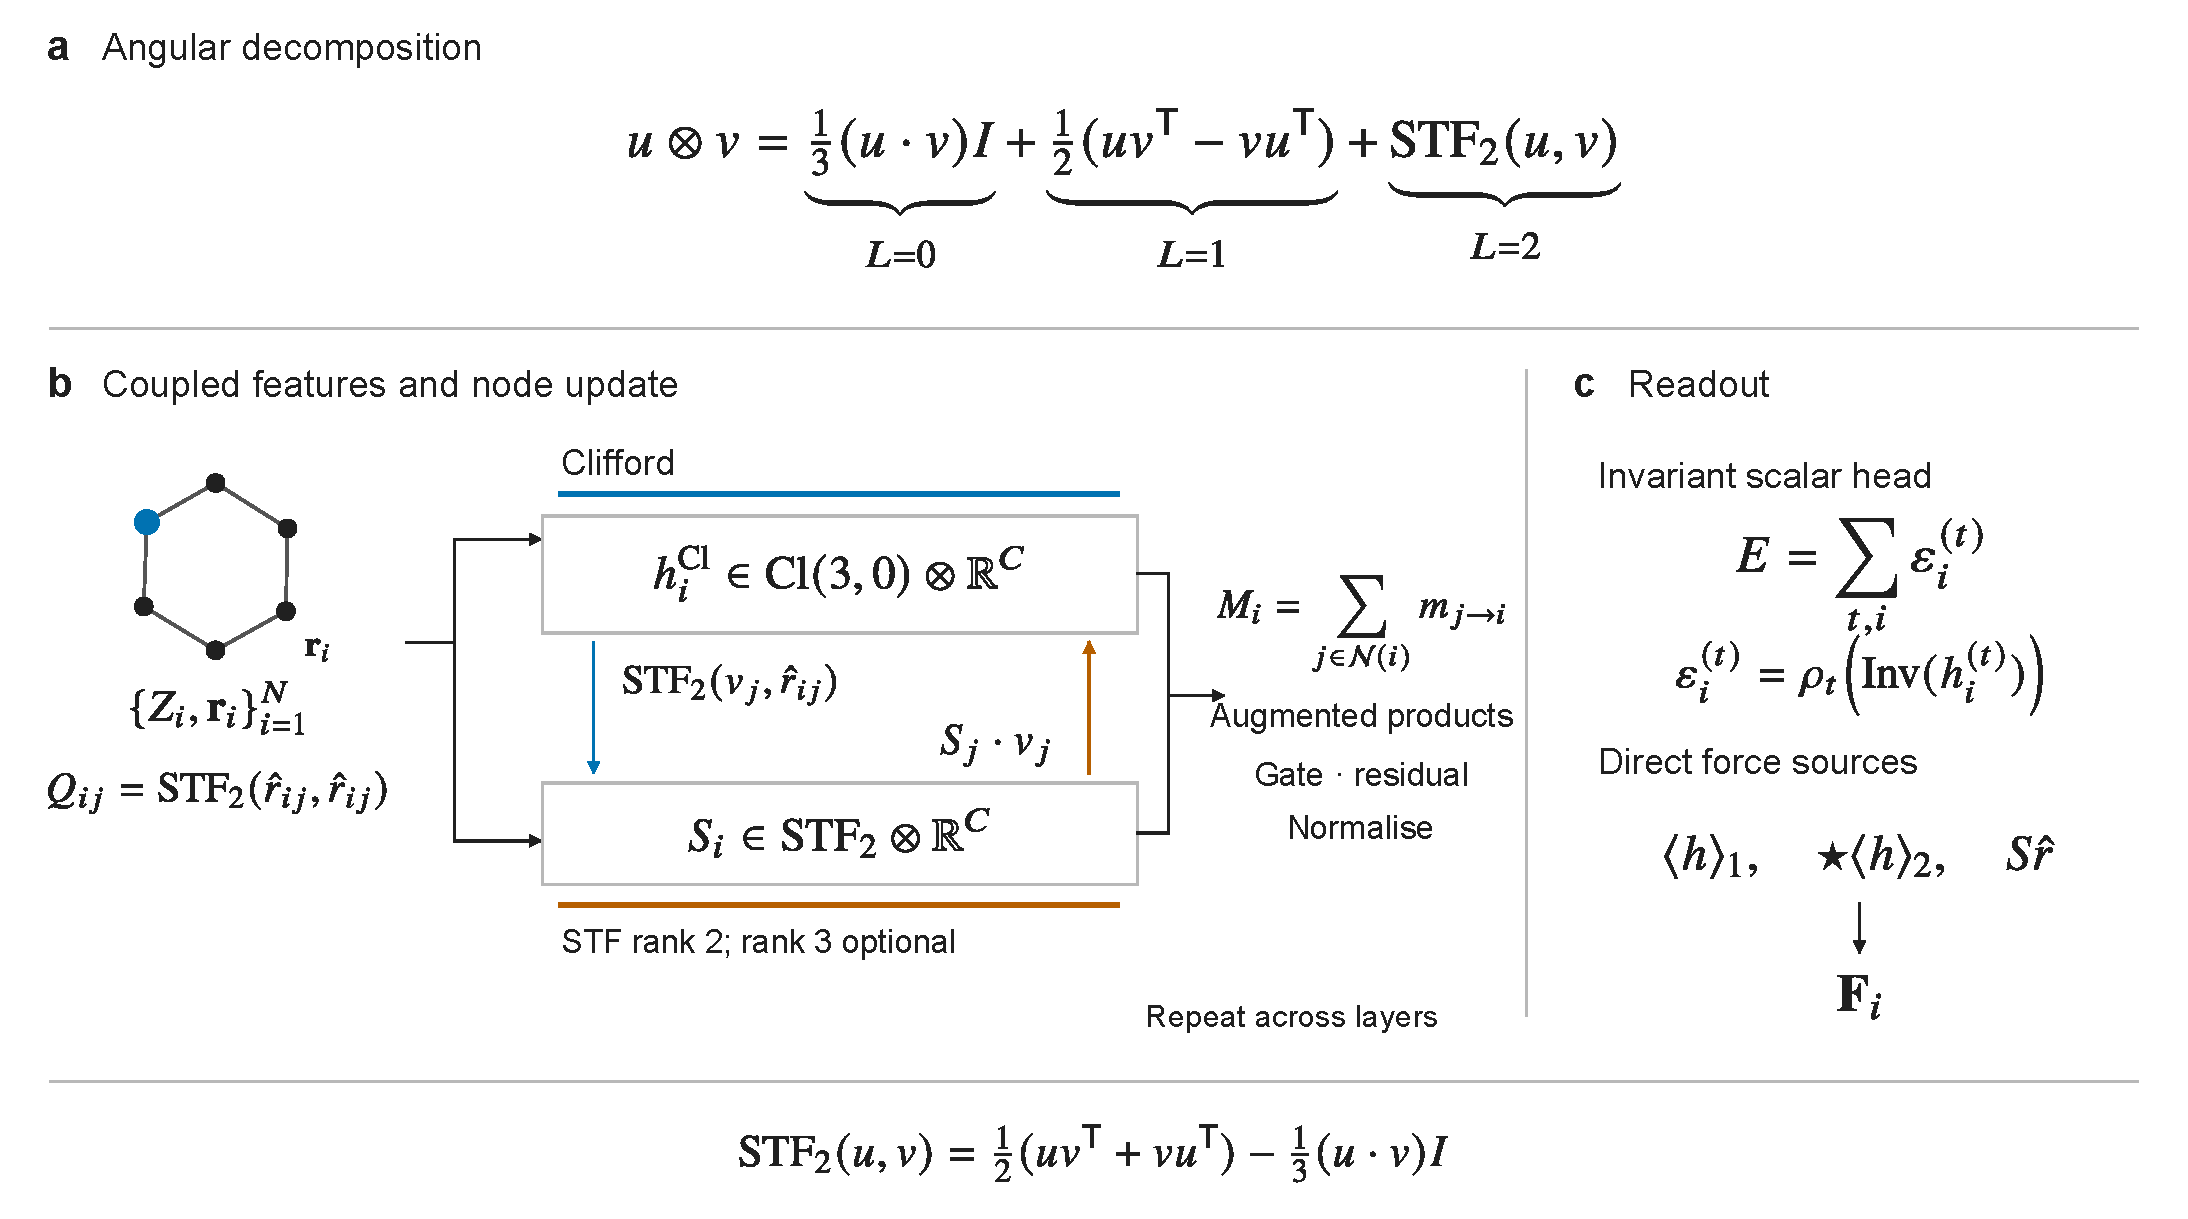
\includegraphics[width=\textwidth]{figures/fig1.pdf}
\caption{\textbf{Angular decomposition and the CliffordSTF architecture.} (a) The vector outer product separates into $L{=}0,1,2$ components (eqn~(\ref{eq:decomp})); the STF projector supplies the symmetric traceless rank-2 part \cite{simeon2023tensornet}. (b) Clifford and STF features exchange information through generation, $\mathrm{STF}_2(v_j,\hat r_{ij})$, and contraction, $S_j\cdot v_j$. Aggregated messages enter augmented products, gating, residual updates and normalisation. Here $v_j$ is the grade-1 feature, $S_j$ the rank-2 STF feature, and $C$ the channel count; rank-3 features are optional. (c) Invariant features feed the energy head, while vector, Hodge-dual and STF-contraction sources feed the direct force head.}
\label{fig:architecture}
\end{figure*}

Machine-learned interatomic potentials (MLIPs) provide practical surrogates for electronic-structure calculations, enabling molecular dynamics at scales beyond direct density functional theory \cite{unke2021machine}. The energy is invariant under rigid rotations and translations, while forces rotate with the atomic configuration and remain unchanged by translation \cite{park2021gnnff}. Force accuracy is commonly assessed through component-wise mean absolute error (MAE), but this metric does not separately identify directional agreement, and low force error alone does not establish simulation quality \cite{fu2023forces}.

Equivariant architectures commonly combine spherical-harmonic features through Clebsch--Gordan (CG) tensor products \cite{thomas2018tensor}. Cartesian alternatives perform equivariant operations directly on tensor features \cite{simeon2023tensornet,zaverkin2024ictp}. Geometric-algebra networks instead use multivectors containing scalars, vectors, oriented planes and oriented volumes, with the geometric product providing a closed-form operation for equivariant message passing \cite{ruhe2023cgenn}.

The classical vector-product decompositions distinguish the scalar and bivector output of the geometric product from the additional rank-2 symmetric traceless component of the outer product \cite{doran2003geometric,coope1965irreducible}. The latter carries angular momentum $L{=}2$, whereas the $\mathrm{Cl}(3,0)$ multivector contains only $L{=}0$ and $L{=}1$ representations \cite{lounesto2001clifford,varshalovich1988quantum}. This suggests a direct architectural question: can supplying the missing angular channels improve the forces predicted by a Clifford potential? CliffordIP \cite{polat2026cliffordip} reaches an aggregate force MAE of $0.021$\,eV\,\AA$^{-1}$ but a force cosine similarity of only $0.051$, providing a concrete setting in which to test this question.

We introduce \textbf{CliffordSTF} (Fig. \ref{fig:architecture}), which couples the Clifford multivector to symmetric traceless tensor (STF) tracks at ranks two and three through closed-form generation and contraction operations. The geometric product retains the Clifford substrate, while the STF operations introduce explicit higher-order angular features. We make three contributions:
\begin{itemize}
\item \textbf{Construction.} We combine the geometric product with classical STF projectors to recover the vector--vector CG decomposition and implement higher-order couplings through $L{=}3$, with learned maps shared across the components of each rotational representation.
\item \textbf{Mechanistic evidence.} Eleven variants plus the CliffordIP baseline isolate the role of the added features. A rank-2 edge descriptor accounts for most of the directional improvement, while the full architecture tests the additional roles of node tracks, cross-track coupling and readout.
\item \textbf{Evaluation.} CliffordSTF raises aggregate rMD17 \cite{rmd17} force cosine from $0.051$ to $0.507$ and lowers force MAE on all ten molecules. OC20 \cite{chanussot2021oc20} and OC22 \cite{tran2023oc22} test transfer to periodic systems, and larger models evaluated with energy-gradient forces demonstrate the performance attainable under longer training recipes.
\end{itemize}

\section{Background: the geometric product and angular momentum}\label{sec:background}

\textbf{Multivectors.} The algebra $\mathrm{Cl}(3,0)$ is generated by orthonormal basis vectors $e_1,e_2,e_3$ with $e_i^2=1$ and $e_ie_j=-e_je_i$ for $i\neq j$ \cite{lounesto2001clifford}. Its $2^3=8$ basis elements are graded by the number of vectors multiplied together: one scalar (grade 0), three vectors $e_i$ (grade 1), three bivectors $e_ie_j$ representing oriented planes (grade 2), and one pseudoscalar $e_1e_2e_3$ representing an oriented volume (grade 3), with a multivector being a linear combination of all eight \cite{ruhe2023gcan}.

\textbf{The geometric product.} For two vectors $u,v$ the geometric product splits into a symmetric and an antisymmetric part \cite{brandstetter2022clifford},
\begin{equation}
uv = u\cdot v + u\wedge v ,
\label{eq:gp}
\end{equation}
a scalar plus a bivector. In three dimensions the Hodge dual maps the bivector $u\wedge v$ to the vector $u\times v$ \cite{doran2003geometric}. The same product applies uniformly to multivectors of any grade and commutes with rotations, enabling equivariant Clifford network operations \cite{ruhe2023cgenn}.

\textbf{Angular momentum.} An irreducible $\mathrm{SO}(3)$ feature of order $L$ has $2L{+}1$ components: scalars are $L{=}0$, vectors are $L{=}1$, and symmetric traceless $3\times3$ matrices are $L{=}2$ \cite{varshalovich1988quantum}. The outer product of two vectors has the classical Cartesian decomposition \cite{coope1965irreducible}
\begin{equation}
u_iv_j = \underbrace{\tfrac13\delta_{ij}\,u\cdot v}_{L=0} + \underbrace{\tfrac12(u_iv_j-u_jv_i)}_{L=1} + \underbrace{\tfrac12(u_iv_j+u_jv_i)-\tfrac13\delta_{ij}\,u\cdot v}_{L=2} .
\label{eq:decomp}
\end{equation}
Comparing eqn~(\ref{eq:gp}) and (\ref{eq:decomp}): the scalar $u\cdot v$ is the $L{=}0$ term and the bivector $u\wedge v$ is the $L{=}1$ term, but the geometric product omits the symmetric traceless $L{=}2$ matrix component used in Cartesian tensor representations \cite{simeon2023tensornet}. Bivectors carry the axial $L{=}1$ representation despite having grade 2 \cite{geiger2022e3nn}; applying the scalar, vector and dual transformation rules to the graded components gives
\begin{equation}
\mathrm{Cl}(3,0) \cong 2\cdot(L{=}0) \oplus 2\cdot(L{=}1), \qquad L{=}2 \notin \mathrm{Cl}(3,0) .
\label{eq:cl_irreps}
\end{equation}
The $L{=}2$ term of eqn~(\ref{eq:decomp}) is exactly the symmetric traceless projection that CliffordSTF adds in closed form. A fuller account of the algebra is given in ESI Section~\ref{E-supp:prelim}.

\section{Related work}\label{sec:related}

\paragraph{Equivariant interatomic potentials.}
SchNet \cite{schutt2017schnet} encodes atomic environments through invariant radial features, while DimeNet++ \cite{gasteiger2020dimenetpp} also incorporates angular information. NequIP \cite{batzner2022nequip} propagates equivariant tensor features, MACE \cite{batatia2022mace} builds higher-order correlations, and EquiformerV2 \cite{liao2024equiformerv2} combines equivariant attention with efficient eSCN convolutions \cite{passaro2023escn}. PaiNN \cite{schutt2021painn}, TorchMD-NET \cite{tholke2022torchmdnet} and ViSNet \cite{wang2024visnet} use scalar and vector features; FAENet \cite{duval2023faenet} uses stochastic frame averaging. We use these architectures as points of comparison for extending the Clifford substrate.

\paragraph{Cartesian tensor constructions.}
The equivalence between symmetric traceless Cartesian tensors and spherical irreducible representations is classical \cite{stone2013theory}; recent work provides orthonormal change-of-basis constructions up to rank 9 \cite{shao2025orthonormal}. ICTP \cite{zaverkin2024ictp} uses irreducible Cartesian tensor products, TensorNet \cite{simeon2023tensornet} uses rank-2 tensor operations, CACE \cite{cheng2024cace} formulates the atomic cluster expansion in Cartesian coordinates, and HotPP \cite{wang2024n} propagates tensors of arbitrary rank. GotenNet \cite{aykent2025gotennet} uses geometry-aware tensor attention, while Gaunt tensor products \cite{luo2024gaunt} offer efficient spherical-harmonic couplings. CliffordSTF draws on the same STF foundation as ICTP, but couples it to a parallel Clifford track through explicit generation and contraction maps (ESI Section~\ref{E-supp:ictp}).

\paragraph{Geometric algebra networks.}
Geometric Clifford algebra networks \cite{ruhe2023gcan}, Clifford group equivariant neural networks \cite{ruhe2023cgenn} and Clifford neural layers \cite{brandstetter2022clifford} use multivector representations and geometric products in neural networks. GATr \cite{brehmer2023geometric} uses projective geometric algebra, Clifford-steerable CNNs \cite{zhdanov2024clifford} construct kernels on pseudo-Riemannian manifolds, and Clifford group-equivariant simplicial message passing networks \cite{liu2024csmpn} extend Clifford message passing to simplicial complexes. Our focus is the explicit angular content of the $\mathrm{Cl}(3,0)$ substrate and its extension for interatomic potentials. OC20 reports force cosine similarity alongside force MAE \cite{chanussot2021oc20}. Prediction-error metrics alone can miss differences in molecular simulation behaviour \cite{kovacs2023mace}. We therefore assess directional agreement separately from force MAE on rMD17.

\section{CliffordSTF}\label{sec:method}


\subsection{Angular channels and closed-form couplings}\label{sec:limitation}\label{sec:stf_channels}

CliffordSTF augments the $L{\leq}1$ multivector substrate of Section~\ref{sec:background} with symmetric traceless tensors. A rank-$\ell$ STF tensor in three dimensions has $2\ell+1$ independent components and carries angular momentum $L{=}\ell$ \cite{applequist1989traceless}. We use the classical rank-2 and rank-3 STF projectors \cite{thorne1980multipole}
\begin{align}
\mathrm{STF}_2(u,v)_{ij} &= \tfrac12(u_iv_j+u_jv_i)-\tfrac13(u\cdot v)\delta_{ij}, \\
\mathrm{STF}_3(S,v)_{ijk} &= T^{\mathrm{sym}}_{ijk}-\tfrac15(\delta_{ij}A_k+\delta_{ik}A_j+\delta_{jk}A_i),
\end{align}
where $T^{\mathrm{sym}}_{ijk}=\tfrac13(S_{ij}v_k+S_{ik}v_j+S_{jk}v_i)$ and $A_k=\tfrac23S_{kl}v_l$. The rank-2 and rank-3 tracks store five and seven independent components, respectively; derivations and storage conventions are given in the ESI.

\begin{theorem}[Geometric-product and STF recovery of the vector tensor product]\label{thm:cg_completeness}
For $u,v\in\mathbb{R}^3$, the classical $\mathbf{1}\otimes\mathbf{1}=\mathbf{0}\oplus\mathbf{1}\oplus\mathbf{2}$ decomposition \cite{coope1965irreducible} is recovered, up to basis normalisation, by
\begin{align*}
[u\otimes v]_{L=0}&=\langle uv\rangle_0, & [u\otimes v]_{L=1}&=\star\langle uv\rangle_2, \\
[u\otimes v]_{L=2}&=\mathrm{STF}_2(u,v).
\end{align*}
Here $\langle\cdot\rangle_k$ extracts grade $k$ and $\star$ is the Hodge dual. All three maps are $\mathrm{SO}(3)$-equivariant.
\end{theorem}

The result follows directly from eqn~(\ref{eq:decomp}) and $\star(u\wedge v)=u\times v$. Our construction combines these classical Cartesian tensor maps with the Clifford product; higher-order contractions used for the $\mathbf{2}\otimes\mathbf{1}$, $\mathbf{2}\otimes\mathbf{2}$ and $\mathbf{3}\otimes\mathbf{1}$ couplings, truncated at $L_{\max}{=}3$, are detailed in ESI Section~\ref{E-supp:cg_proof}. Primitive-level Cartesian projector checks and end-to-end rotation tests are described in ESI Section~\ref{E-supp:cg_test}.

\subsection{Architecture}\label{sec:architecture}

Figure~\ref{fig:architecture} shows the two feature tracks. Each atom carries a Clifford multivector (8 components per channel), with optional rank-2 STF features (13 components in total) and rank-3 STF features (20 in total). Disabling the added features and readout paths recovers the CliffordIP baseline, including its layer-dependent schedule for progressively activating multivector grades. The implementation uses standard PyTorch operations \cite{paszke2019pytorch} with an $8\times8$ geometric-product Cayley table and closed-form STF maps.

\textbf{Embedding.} Atomic numbers initialise scalar features through a learned embedding. Radial basis functions modulate edge scalars and direction vectors in the Clifford edge feature $\tilde e_{ij}$. A separate rank-2 edge block carries $\mathrm{STF}_2(\hat r_{ij},\hat r_{ij})$. STF node features are initialised with small Gaussian noise ($\sigma=10^{-3}$); edge construction and architectural settings are specified in ESI Sections~\ref{E-supp:edge_embed} and~\ref{E-supp:protocol}.

\textbf{Message passing.} With $\mathrm{GP}$ denoting the geometric product, the Clifford message is
\begin{align*}
m^{\mathrm{Cl}}_{j\to i}=\alpha_{ij}\bigl[&W_1\cdot\mathrm{GP}(h_j^{\mathrm{Cl}},\tilde e_{ij}) \\
&+W_2\cdot\mathrm{GP}(\tilde e_{ij},h_j^{\mathrm{Cl}})+W_{\mathrm{skip}}\cdot h_j^{(0)}\bigr],
\end{align*}
where $\alpha_{ij}$ is invariant attention computed from scalar features and radial information. The STF tracks generate higher-rank features and propagate existing features through
\begin{align*}
m^{\mathrm{STF}_2}_{j\to i}&=W_g^{(2)}\cdot\mathrm{STF}_2(h_j^{\mathrm{vec}},\hat r_{ij})+\phi(r_{ij})W_p^{(2)}\cdot h_j^{\mathrm{STF}_2}, \\
m^{\mathrm{STF}_3}_{j\to i}&=W_g^{(3)}\cdot\mathrm{STF}_3(h_j^{\mathrm{STF}_2},\hat r_{ij})+\phi(r_{ij})W_p^{(3)}\cdot h_j^{\mathrm{STF}_3},
\end{align*}
with invariant radial weights $\phi$. Every learned linear map mixes channels with the same weights for each component of an irrep: $(W\cdot h)^{(\ell)}_{c,m}=\sum_{c'}W_{cc'}h^{(\ell)}_{c',m}$. This component-shared channel mixing commutes with rotations \cite{shao2025orthonormal}; we apply separate maps to the Clifford grades and STF ranks.

\textbf{Cross-track coupling and updates.} Contracting rank-2 features with Clifford vectors feeds angular information back into the vector track:
\[
m^{\mathrm{Cl}}_{j\to i}[\text{grade-1}]\mathrel{+}=W_{\mathrm{cross}}\cdot(h_j^{\mathrm{STF}_2}\cdot h_j^{\mathrm{vec}}).
\]
Together with generation of STF features from vectors, this provides bidirectional coupling. At the node-update stage, iterated augmented products combine the tracks through the six bilinear terms listed in ESI Section~\ref{E-supp:aug_prod}, providing correlations up to body order four. A block-diagonal channel map, equivariant gating \cite{weiler20183d}, a residual connection \cite{he2016residual} and track-wise normalisation complete the update. Optional invariant gates modulate STF tracks between layers (ESI Sections~\ref{E-supp:normalization} and~\ref{E-supp:routing}).

\subsection{Energy and force readout}\label{sec:readout}

The energy head combines grade-0 scalars, geometric-product self-interaction scalars and STF Frobenius norms in a multilayer perceptron. Summed per-atom, per-layer contributions give the total energy. The direct force head combines grade-1 vectors and Hodge duals of grade-2 bivectors, with a scatter-summed rank-2 contraction $S\hat r$ gated by invariant STF norms. The larger-model experiments instead use energy-gradient forces, following the conservative force formulation \cite{chmiela2017conservative}, with the protocol specified in Section~\ref{sec:seeds}.

\label{rem:so3_vs_o3}All maps are formulated for rotational $\mathrm{SO}(3)$ equivariance. Polar vectors and Hodge-dual axial vectors transform identically under rotations but have different reflection parities \cite{geiger2022e3nn}. ESI Section~\ref{E-supp:so3_o3} gives the resulting requirements for extending our readout to full $\mathrm{O}(3)$ equivariance.

\section{Results and discussion}\label{sec:experiments}

\subsection{Benchmarks and protocol}\label{sec:benchmarks}

The primary benchmark is rMD17, comprising ten small organic molecules with DFT energies and forces. We report energy MAE, component-wise force MAE and force cosine similarity, the mean cosine between predicted and reference atomic force vectors. OC20 and OC22 test transfer to periodic adsorbate--surface systems through structure-to-energy-and-forces (S2EF) and initial-structure-to-relaxed-energy (IS2RE) prediction.

The baseline values in Tables~\ref{tab:rmd17_cip} and~\ref{tab:oc_main} are taken from the published CliffordIP benchmark, which compares architectures at approximately $10^6$ parameters. CliffordSTF ($1.06\times10^6$ parameters) follows its data splits and training recipe: Adam \cite{kingma2015adam} at a constant learning rate of $10^{-4}$, no weight decay, no weight averaging or warm-up, and early stopping with patience 30. CliffordSTF additionally clips the gradient norm at 10 and uses a longer OC22 IS2RE epoch budget; full settings are in ESI Section~\ref{E-supp:protocol}. We average all CliffordSTF seeds: four on rMD17 and OC22, and three on OC20. The primary experiments use the direct force head; the larger-model comparison in Section~\ref{sec:seeds} uses energy-gradient forces to match the force formulation of its reference comparison.

\subsection{Force prediction on rMD17}\label{sec:cliffordip}

CliffordSTF lowers aggregate force MAE from $0.021$ to $0.018$\,eV\,\AA$^{-1}$ relative to CliffordIP, with lower error on every molecule (Table~\ref{tab:rmd17_cip}). Aggregate energy MAE remains $0.034$\,eV at the reported precision. Force cosine similarity increases from $0.051$ to $0.507$, indicating substantially better directional agreement under this protocol. CliffordSTF has the lowest force MAE among the sixteen models shown in the table; FAENet has the lowest aggregate energy MAE.

% BEGIN GENERATED TABLE: tab_rmd17_permol
\begin{table*}[t]
\centering
\caption{\textbf{rMD17 test MAE per molecule.} Mean over four seeds; $f$: force MAE (eV\,\AA$^{-1}$), $e$: energy MAE (eV), Agg.: mean over ten molecules. Best value among the models shown per metric and column in bold. Baselines from ref.~\citenum{polat2026cliffordip}; protocol details are given in Section~\ref{sec:cliffordip} and ESI Section~\ref{E-supp:protocol}.}
\label{tab:rmd17_cip}
\fontsize{8.5}{9.6}\selectfont
\setlength{\tabcolsep}{2.4pt}
\renewcommand{\arraystretch}{1.02}
\begin{tabular*}{\textwidth}{@{\extracolsep{\fill}}llrrrrrrrrrrr@{}}
\toprule
Model & & Asp & Azo & Bnz & Eth & Mal & Nap & Par & Sal & Tol & Ura & Agg. \\
\midrule
\textbf{CliffordSTF} (this work) & $f$ & \textbf{0.021} & \textbf{0.019} & \textbf{0.009} & \textbf{0.015} & \textbf{0.018} & \textbf{0.018} & \textbf{0.020} & \textbf{0.020} & \textbf{0.017} & \textbf{0.021} & \textbf{0.018} \\
 & $e$ & \textbf{0.028} & 0.038 & 0.028 & 0.011 & 0.026 & 0.019 & 0.058 & \textbf{0.037} & 0.055 & 0.037 & 0.034 \\
\addlinespace[1pt]
FAENet & $f$ & 0.022 & 0.022 & 0.011 & 0.020 & 0.020 & 0.022 & 0.025 & 0.022 & 0.021 & 0.022 & 0.021 \\
 & $e$ & 0.033 & \textbf{0.034} & \textbf{0.004} & \textbf{0.003} & \textbf{0.004} & 0.037 & 0.073 & 0.038 & \textbf{0.008} & \textbf{0.005} & \textbf{0.024} \\
\addlinespace[1pt]
CliffordIP & $f$ & 0.022 & 0.022 & 0.015 & 0.020 & 0.022 & 0.021 & 0.021 & 0.022 & 0.021 & 0.022 & 0.021 \\
 & $e$ & 0.070 & 0.053 & 0.034 & 0.014 & 0.032 & \textbf{0.013} & \textbf{0.025} & \textbf{0.037} & 0.037 & 0.023 & 0.034 \\
\addlinespace[1pt]
TorchMD-Net & $f$ & 0.625 & 0.356 & 0.155 & 0.152 & 0.291 & 0.241 & 0.466 & 0.377 & 0.233 & 0.282 & 0.318 \\
 & $e$ & 1.580 & 0.716 & 0.246 & 0.165 & 0.509 & 0.637 & 1.334 & 0.829 & 0.219 & 0.878 & 0.711 \\
\addlinespace[1pt]
SchNet & $f$ & 1.273 & 0.903 & 0.202 & 0.095 & 0.230 & 0.679 & 1.375 & 1.169 & 0.606 & 0.658 & 0.719 \\
 & $e$ & 1.664 & 1.465 & 0.622 & 0.321 & 0.502 & 1.376 & 1.571 & 1.922 & 0.590 & 1.292 & 1.132 \\
\addlinespace[1pt]
DimeNet++ & $f$ & 1.157 & 0.937 & 0.303 & 0.374 & 0.736 & 0.628 & 1.069 & 0.984 & 0.531 & 0.931 & 0.765 \\
 & $e$ & 2.824 & 3.549 & 0.258 & 0.484 & 1.136 & 1.003 & 0.935 & 1.293 & 0.677 & 1.096 & 1.326 \\
\addlinespace[1pt]
PaiNN & $f$ & 1.390 & 1.082 & 0.412 & 0.384 & 0.716 & 0.798 & 0.942 & 0.984 & 0.709 & 1.069 & 0.849 \\
 & $e$ & 3.886 & 2.862 & 0.602 & 0.553 & 1.551 & 1.156 & 2.455 & 0.759 & 1.089 & 1.944 & 1.686 \\
\addlinespace[1pt]
ViSNet & $f$ & 1.638 & 1.386 & 0.484 & 0.463 & 0.741 & 0.776 & 1.067 & 1.192 & 0.625 & 0.977 & 0.935 \\
 & $e$ & 4.953 & 5.037 & 0.351 & 1.207 & 0.518 & 1.940 & 3.296 & 3.319 & 0.903 & 2.303 & 2.383 \\
\addlinespace[1pt]
NequIP & $f$ & 6.101 & 2.708 & 1.203 & 1.220 & 2.425 & 1.834 & 4.383 & 2.921 & 1.092 & 2.511 & 2.640 \\
 & $e$ & 3.673 & 1.049 & 0.193 & 0.448 & 0.950 & 0.584 & 3.061 & 1.195 & 0.398 & 0.737 & 1.229 \\
\addlinespace[1pt]
MACE $L{=}3$ & $f$ & 6.971 & 4.379 & 1.060 & 1.386 & 2.495 & 3.072 & 4.666 & 5.602 & 2.509 & 4.306 & 3.645 \\
 & $e$ & 2.813 & 1.600 & 0.214 & 0.411 & 0.755 & 0.906 & 2.163 & 1.838 & 0.931 & 1.197 & 1.283 \\
\addlinespace[1pt]
MACE $L{=}2$ & $f$ & 8.532 & 5.172 & 1.328 & 2.115 & 2.899 & 4.858 & 6.627 & 6.753 & 3.863 & 4.498 & 4.664 \\
 & $e$ & 4.210 & 1.942 & 0.364 & 0.643 & 0.876 & 1.737 & 3.087 & 2.303 & 1.514 & 1.338 & 1.801 \\
\addlinespace[1pt]
ICTP $L{=}2$ & $f$ & 7.972 & 6.098 & 2.271 & 1.736 & 2.448 & 5.452 & 7.500 & 7.615 & 3.188 & 5.804 & 5.008 \\
 & $e$ & 3.464 & 2.720 & 0.370 & 0.451 & 0.695 & 2.066 & 3.898 & 2.779 & 1.280 & 1.740 & 1.946 \\
\addlinespace[1pt]
ICTP $L{=}1$ & $f$ & 9.347 & 5.261 & 1.923 & 2.201 & 3.788 & 5.028 & 8.120 & 8.106 & 3.247 & 4.146 & 5.117 \\
 & $e$ & 4.493 & 2.103 & 0.576 & 0.740 & 1.141 & 2.102 & 4.368 & 3.367 & 1.534 & 1.256 & 2.168 \\
\addlinespace[1pt]
ICTP $L{=}3$ & $f$ & 11.822 & 6.691 & 1.450 & 1.951 & 3.524 & 5.236 & 7.776 & 7.786 & 3.215 & 3.113 & 5.256 \\
 & $e$ & 5.704 & 2.774 & 0.315 & 0.556 & 0.973 & 1.797 & 3.281 & 2.934 & 1.049 & 0.920 & 2.030 \\
\addlinespace[1pt]
MACE $L{=}1$ & $f$ & 10.412 & 5.577 & 2.517 & 2.186 & 4.310 & 6.521 & 6.311 & 7.371 & 5.019 & 6.089 & 5.631 \\
 & $e$ & 5.019 & 2.209 & 0.445 & 0.753 & 1.311 & 2.437 & 2.806 & 2.940 & 2.182 & 1.821 & 2.192 \\
\addlinespace[1pt]
GotenNet & $f$ & 21.637 & 4.789 & 10.636 & 1.787 & 13.962 & 3.898 & 6.759 & 4.183 & 2.574 & 11.292 & 8.152 \\
 & $e$ & 16.337 & 4.267 & 15.159 & 1.422 & 87.421 & 2.416 & 40.971 & 41.686 & 39.698 & 28.193 & 27.757 \\
\bottomrule
\end{tabular*}
\end{table*}
% END GENERATED TABLE: tab_rmd17_permol

\subsection{What drives the directional gain}\label{sec:ablation}

Eleven variants plus the CliffordIP baseline isolate the added components on four rMD17 molecules. Table~\ref{tab:ablation} shows the key comparisons; the complete flag matrix and results are in ESI Section~\ref{E-supp:variants}. Adding only the $L{=}2$ edge descriptor $\mathrm{STF}_2(\hat r_{ij},\hat r_{ij})$ raises force cosine from $0.030$ to $0.498$, close to the full model's $0.506$. Explicit rank-2 information entering message passing therefore accounts for most of the measured directional improvement. The full model has the highest mean cosine, while adding Hodge readout to the edge-only configuration gives the lowest force MAE.

The readout comparison identifies how that information is used. Retaining the STF message-passing paths but reading forces from STF channels alone lowers cosine to $0.097$. In the tested configurations, the directional gain is realised when the angularly enriched messages are read out through Clifford vector channels. Node tracks, routing and cross-track coupling produce smaller, configuration-dependent changes. The Full no cross runs also disable routing; their per-seed stability analysis is reported in ESI Section~\ref{E-supp:cross_stability}.

% BEGIN GENERATED TABLE: tab_ablation
\begin{table*}[t]
\centering
\caption{\textbf{Key rMD17 ablations.} Mean $\pm$ standard deviation over six seeds, averaging aspirin, benzene, ethanol and salicylic acid within each seed; approximately $10^6$ parameters per variant. All variants except the baseline use the rank-2 edge descriptor. Bold marks the best mean in the full ablation; all eleven variants plus the baseline and their flags are in ESI Table~\ref{E-tab:ablation_full}.}
\label{tab:ablation}
\fontsize{8.5}{10}\selectfont
\setlength{\tabcolsep}{3pt}
\begin{tabular*}{\textwidth}{@{\extracolsep{\fill}}llrrr@{}}
\toprule
Variant & STF node ranks & Force cosine $\uparrow$ & Force MAE (meV\,\AA$^{-1}$) & Energy MAE (meV) \\
\midrule
CliffordIP baseline & None & 0.030 $\pm$ 0.003 & 19.704 $\pm$ 0.043 & 125.848 $\pm$ 77.191 \\
Rank-2 edge only & None & 0.498 $\pm$ 0.084 & 17.221 $\pm$ 0.537 & 26.294 $\pm$ 8.464 \\
Rank-2 edge + Hodge readout & None & 0.472 $\pm$ 0.103 & \textbf{16.584} $\pm$ 1.166 & 30.975 $\pm$ 13.434 \\
STF tracks, no routing & 2, 3 & 0.489 $\pm$ 0.119 & 17.029 $\pm$ 1.016 & 36.792 $\pm$ 9.466 \\
Full, no cross or routing & 2, 3 & 0.474 $\pm$ 0.072 & 17.170 $\pm$ 0.674 & 70.409 $\pm$ 92.001 \\
Full CliffordSTF & 2, 3 & \textbf{0.506} $\pm$ 0.045 & 16.802 $\pm$ 0.556 & 45.986 $\pm$ 48.658 \\
STF-only readout & 2, 3 & 0.097 $\pm$ 0.028 & 19.545 $\pm$ 0.098 & 36.640 $\pm$ 39.015 \\
\bottomrule
\end{tabular*}
\end{table*}
% END GENERATED TABLE: tab_ablation

\subsection{Transfer to periodic catalysis}\label{sec:catalysis}

On OC20, the added channels improve both relaxed-energy prediction and forces relative to CliffordIP (Table~\ref{tab:oc_main}). IS2RE energy MAE decreases on all four validation splits, including $0.77$ to $0.70$\,eV in distribution. S2EF force MAE decreases from $0.064$ to $0.060$\,eV\,\AA$^{-1}$, and the unseen-catalyst energy errors ($2.84$\,eV on OOD-Cat. and $3.49$\,eV on OOD-Both) are the lowest in this comparison. CliffordIP retains lower S2EF energy error in distribution and on unseen adsorbates; EquiformerV2 $L{=}2$ retains lower force MAE.

On OC22 S2EF, CliffordSTF matches CliffordIP's force MAE ($0.073$\,eV\,\AA$^{-1}$) with similar in-distribution energy error ($2.92$ versus $2.89$\,eV). Directional improvements over CliffordIP are modest on both periodic datasets, and other baselines retain higher force cosine (ESI Tables~\ref{E-tab:oc20_full} and~\ref{E-tab:oc22_full}). OC22 IS2RE remains weaker: the all-seed in-distribution mean is $6.39$\,eV versus CliffordIP's $3.47$\,eV, including one early-diverging run; the other three seeds average $4.09$\,eV. Full splits and seed statistics are retained in ESI Section~\ref{E-supp:oc_full}.

% BEGIN GENERATED TABLE: tab_oc_main
\begin{table*}[t]
\centering
\caption{\textbf{OC20 and OC22 validation results} (mean $\pm$ standard deviation over seeds; best value per column in bold, second best underlined). Baselines from ref.~\citenum{polat2026cliffordip}; protocol in Section~\ref{sec:benchmarks}. CliffordSTF averages all seeds (3 on OC20, 4 on OC22). Energy MAE in eV, force MAE in eV\,\AA$^{-1}$. Force cosine similarity, the remaining IS2RE splits, OC22 out-of-distribution energy and OC22 IS2RE are in ESI Tables~\ref{E-tab:oc20_full}--\ref{E-tab:oc22_full}.}
\label{tab:oc_main}
\setlength{\tabcolsep}{3pt}
\resizebox{\textwidth}{!}{%
\begin{tabular}{lccccccccc}
\toprule
& \multicolumn{5}{c}{OC20 S2EF} & \multicolumn{2}{c}{OC20 IS2RE} & \multicolumn{2}{c}{OC22 S2EF} \\
\cmidrule(lr){2-6}\cmidrule(lr){7-8}\cmidrule(lr){9-10}
Model & $e$ ID & $e$ OOD-Ads. & $e$ OOD-Cat. & $e$ OOD-Both & $f$ ID & ID & OOD-Both & $e$ ID & $f$ ID \\
\midrule
\textbf{CliffordSTF} (this work) & \underline{2.11} $\pm$ 0.05 & \underline{2.21} $\pm$ 0.06 & \textbf{2.84} $\pm$ 0.11 & \textbf{3.49} $\pm$ 0.13 & \underline{0.060} $\pm$ 0.000 & 0.70 $\pm$ 0.01 & 0.75 $\pm$ 0.02 & \underline{2.92} $\pm$ 0.11 & \underline{0.073} $\pm$ 0.000 \\
\midrule
SchNet & 4.77 $\pm$ 0.05 & 4.82 $\pm$ 0.08 & 4.85 $\pm$ 0.08 & 5.83 $\pm$ 0.08 & 0.070 $\pm$ 0.001 & 0.77 $\pm$ 0.01 & 0.80 $\pm$ 0.04 & 7.35 $\pm$ 0.99 & 0.077 $\pm$ 0.001 \\
DimeNet++ & 4.10 $\pm$ 0.01 & 4.16 $\pm$ 0.00 & 4.47 $\pm$ 0.00 & 5.37 $\pm$ 0.03 & 0.063 $\pm$ 0.000 & 0.70 $\pm$ 0.01 & 0.77 $\pm$ 0.02 & 5.36 $\pm$ 0.10 & 0.075 $\pm$ 0.000 \\
PaiNN & 4.22 $\pm$ 0.03 & 4.29 $\pm$ 0.04 & 4.45 $\pm$ 0.01 & 5.34 $\pm$ 0.01 & 0.066 $\pm$ 0.000 & 0.72 $\pm$ 0.01 & 0.83 $\pm$ 0.04 & 5.41 $\pm$ 0.14 & 0.076 $\pm$ 0.000 \\
TorchMD-Net & 3.71 $\pm$ 0.01 & 3.76 $\pm$ 0.01 & 4.15 $\pm$ 0.01 & 4.94 $\pm$ 0.01 & 0.064 $\pm$ 0.000 & 0.72 $\pm$ 0.01 & 0.74 $\pm$ 0.04 & 4.28 $\pm$ 0.00 & 0.075 $\pm$ 0.000 \\
NequIP & 5.75 $\pm$ 0.08 & 5.81 $\pm$ 0.08 & 5.90 $\pm$ 0.02 & 7.12 $\pm$ 0.01 & 0.077 $\pm$ 0.000 & 0.93 $\pm$ 0.03 & 0.90 $\pm$ 0.05 & 9.90 $\pm$ 0.09 & 0.079 $\pm$ 0.000 \\
GotenNet & 3.56 $\pm$ 0.20 & 3.65 $\pm$ 0.17 & 3.96 $\pm$ 0.13 & 4.77 $\pm$ 0.15 & 0.063 $\pm$ 0.002 & \underline{0.69} $\pm$ 0.01 & \textbf{0.71} $\pm$ 0.04 & 4.52 $\pm$ 0.28 & \underline{0.073} $\pm$ 0.000 \\
EquiformerV2 $L{=}2$ & 2.47 $\pm$ 0.08 & 2.52 $\pm$ 0.09 & 2.96 $\pm$ 0.10 & 3.62 $\pm$ 0.12 & \textbf{0.059} $\pm$ 0.001 & \textbf{0.65} $\pm$ 0.01 & \underline{0.72} $\pm$ 0.02 & 3.13 $\pm$ 0.18 & \textbf{0.072} $\pm$ 0.000 \\
EquiformerV2 $L{=}4$ & 2.37 $\pm$ 0.12 & 2.42 $\pm$ 0.12 & \underline{2.89} $\pm$ 0.10 & \underline{3.51} $\pm$ 0.15 & \underline{0.060} $\pm$ 0.000 & 0.77 $\pm$ 0.10 & 0.78 $\pm$ 0.05 & 3.38 $\pm$ 0.04 & \textbf{0.072} $\pm$ 0.000 \\
MACE $L{=}1$ & 5.88 $\pm$ 0.25 & 5.93 $\pm$ 0.24 & 6.02 $\pm$ 0.15 & 7.11 $\pm$ 0.19 & 0.077 $\pm$ 0.000 & 0.97 $\pm$ 0.10 & 0.97 $\pm$ 0.02 & 10.11 $\pm$ 0.14 & 0.078 $\pm$ 0.000 \\
MACE $L{=}2$ & 6.04 $\pm$ 0.33 & 6.07 $\pm$ 0.32 & 6.10 $\pm$ 0.28 & 7.15 $\pm$ 0.30 & 0.075 $\pm$ 0.000 & 0.92 $\pm$ 0.08 & 0.86 $\pm$ 0.08 & 10.26 $\pm$ 0.41 & 0.078 $\pm$ 0.000 \\
ICTP $L{=}1$ & 6.00 $\pm$ 0.09 & 6.09 $\pm$ 0.10 & 5.92 $\pm$ 0.09 & 7.19 $\pm$ 0.08 & 0.078 $\pm$ 0.002 & 0.88 $\pm$ 0.01 & 0.88 $\pm$ 0.04 & 11.70 $\pm$ 0.59 & 0.080 $\pm$ 0.001 \\
ICTP $L{=}2$ & 6.64 $\pm$ 0.31 & 6.68 $\pm$ 0.30 & 6.50 $\pm$ 0.33 & 7.85 $\pm$ 0.37 & 0.077 $\pm$ 0.000 & 0.88 $\pm$ 0.02 & 0.93 $\pm$ 0.06 & 12.37 $\pm$ 0.23 & 0.081 $\pm$ 0.001 \\
CliffordIP & \textbf{1.89} $\pm$ 0.01 & \textbf{1.98} $\pm$ 0.01 & 2.96 $\pm$ 0.03 & \underline{3.51} $\pm$ 0.00 & 0.064 $\pm$ 0.000 & 0.77 $\pm$ 0.02 & 0.85 $\pm$ 0.02 & \textbf{2.89} $\pm$ 0.21 & \underline{0.073} $\pm$ 0.000 \\
\bottomrule
\end{tabular}%
}
\end{table*}
% END GENERATED TABLE: tab_oc_main

\subsection{Larger models with energy-gradient forces}\label{sec:seeds}

We evaluate two larger CliffordSTF configurations on all ten rMD17 molecules with four seeds each, using forces $F=-\partial E/\partial x$ to match the energy-gradient formulation of the published comparison \cite{aykent2025gotennet}. We use the released default rMD17 configuration for CliffordSTF-1.9M and a cosine learning-rate schedule with a larger model for CliffordSTF-10M (ESI Section~\ref{E-supp:published}). Their full training settings and published reference values are given in ESI Section~\ref{E-supp:published}.

Across these configurations, seed-mean force MAE falls on every molecule by a factor of $2.0$--$6.2$, with median error decreasing from $0.732$ to $0.208$\,kcal\,mol$^{-1}$\,\AA$^{-1}$. These results reflect changes in capacity and training recipe together. Mean force cosine lies between $0.9954$ and $1.0000$ across all 80 held-out evaluations. The per-seed results, stopping-epoch analysis and comparison with published force errors are provided in the ESI.

\subsection{Computational cost}\label{sec:cost}

On rMD17 aspirin at approximately $10^6$ parameters, CliffordSTF takes $0.352$\,s per inference step and $7.77$\,s per training step, compared with $0.128$ and $3.11$\,s for CliffordIP under the timing protocol. Inference is comparable to ICTP $L{=}2/3$, and training takes $1.25\times$ the time of ICTP $L{=}3$. In the separate memory measurement, CliffordSTF uses $20\%$ more inference memory and $32\%$ more training memory than CliffordIP. Hardware, batch sizes, model sizes and the complete measurements are reported in ESI Sections~\ref{E-supp:published} and~\ref{E-supp:wallclock}.

\section{Discussion and limitations}\label{sec:limitations}

CliffordSTF provides a closed-form route from a Clifford potential to explicit higher-order angular features. The ablation identifies the rank-2 edge descriptor as the main source of the directional gain under the evaluated protocol, with STF node tracks and cross-track coupling providing additional architectural choices. The resulting design preserves geometric-product message passing while making the contribution of the added angular information directly testable.

The evidence is strongest for small organic molecules under the rMD17 protocols studied here. At the primary training budget, force cosine reaches $0.507$; the larger configurations attain values above $0.995$ with energy-gradient forces and longer recipes, while leading published models retain lower force MAE. Periodic-system results are mixed: OC20 improves over CliffordIP, but OC22 IS2RE remains weaker, including one divergent seed. The full model also incurs additional training time and memory, and the cost of the simpler edge-only variant has not been measured separately. The present construction carries angular orders through $L{=}3$ and guarantees rotational $\mathrm{SO}(3)$ equivariance; reflection equivariance would require explicit parity tracking. The results support adding explicit angular channels to this Clifford backbone. Broader chemical coverage and lower-cost implementations remain to be evaluated.


\section*{Conclusions}

CliffordSTF extends geometric-product message passing with explicit symmetric traceless angular channels. A rank-2 edge descriptor supplies most of the directional improvement observed in the controlled rMD17 ablation, while the coupled architecture provides a systematic way to propagate and read out higher-order information. This connects the compact Clifford substrate with Cartesian tensor representations and helps identify which angular features to add to a Clifford interatomic potential.

\section*{Author contributions}

C.P. conceived and implemented CliffordSTF and its training pipeline, conducted the training runs and benchmark experiments, performed the data analysis, and wrote the original manuscript. M.K. supervised the research, evaluated and validated the materials-science aspects of the study, contributed to the interpretation of the data and results, and reviewed and edited the manuscript. E.S. provided resources, contributed to the supervision of the research, and reviewed and edited the manuscript. H.K. contributed to the supervision of the research, interpretation of the results, and review and editing of the manuscript. All authors read and approved the final manuscript.

\section*{Conflicts of interest}

There are no conflicts to declare.

\section*{Data availability}

The rMD17 \cite{christensen2020role}, OC20 \cite{chanussot2021oc20} and OC22 \cite{tran2023oc22} datasets are publicly available from their original sources. Baseline values are taken from the published CliffordIP study \cite{polat2026cliffordip} and from ref.~\citenum{aykent2025gotennet}. The PyTorch implementation of CliffordSTF, the per-benchmark configurations, the evaluation script, every per-seed CliffordSTF result, the 80 held-out rMD17 evaluations with their stopping epochs, and the scripts that generate the manuscript and ESI tables and figures are available at \url{https://github.com/KurbanIntelligenceLab/CliffordSTF}.

\section*{Acknowledgements}

No funding was received for this research.

\makeatletter
\if@firstcolumn
  \balance
\else
  \AddToHookNext{shipout/after}{\balance}
\fi
\makeatother

\renewcommand\refname{Notes and references}

\bibliography{main}
\bibliographystyle{rsc-local}

\end{document}
